%%%%%%%%%%%%%%%%%%%%%%%%%%%%%%%%%%%%%%%%%%%%%%%%%%%%%%%%%%%%%%%%%%%%%%%%%%%%%%%%
% Diese Datei beinhaltet den eigentlichen Inhalt Ihrer Arbeit.
%
% Es bietet sich der Übersicht halber an, die einzelnen Abschnitte jeweils
% in eigene Dateien zu schreiben und mittels \input einzubinden.
% Eine mögliche Verzeichnisstruktur sähe entsprechend so aus:
%
% thesis/
% +- tex/
% |  +- introduction.tex
% |  +- motivation.tex
% |  +- experiments.tex
% |  |  ...
% |  +- conclusion.tex
% +- abstract.tex
% +- contents.tex
% +- thesis.tex
%%%%%%%%%%%%%%%%%%%%%%%%%%%%%%%%%%%%%%%%%%%%%%%%%%%%%%%%%%%%%%%%%%%%%%%%%%%%%%%%

\section{Introduction}

Over the decades since its inception, the field of computer science has become increasingly complex and confusing.
This has caused students today to lose track of the picture at large and instead specialize on specific aspects of the field.
Shimon Schocken and Noam Nisam believe that this is an issue and that the best way to understand how computers actually work is to build one from scratch yourself.~\cite[Preface]{nisan2005}

In order to enable students to take this seemingly impossible approach, Schocken and Nisan developed the Nand to Tetris course in 2004, which gives students the opportunity to build an entire computer system themselves.~\cite{1408798}
The system the participants create over the course of twelve projects is powerful enough to allow for the implementation of complex applications and games.\ref{fig:hackenstein-offiziell}

To enable students to work on the included projects in a different order than intended, the authors included a hardware simulator to start with and two different emulators, which are capable of emulating the progress of the preceding projects.
Those emulators however are also a frequent point of criticism among course participants, as they increasingly no longer meet the demands of modern users.
Written in Java using the Swing Framework they are not only slow, but also do not adapt to today's higher display resolutions, making it difficult to actually see the contents of the running application.

It is therefore meaningful to rewrite those emulators in order to make the course more approachable and by extension increase the number of participants.

As part of this work, the two emulators were rewritten as a browser application using WebAssembly. This not only enables support for larger screens and significantly improved performance, but also allows the tools to be used without being installed on the the student's computer.

\section{Related work}

\subsection{Nand to Tetris}
\begin{itemize}
  \item VM Bytecode design und high level Funktionalität
  \item CPU Assembly design und high level Funktionalität
  \item TST design und high level Funktionalität
  \item Viele Tests für Emulatoren aus N2T Projekten
\end{itemize}

\subsection{Dependencies}
\begin{itemize}
\item lazy\_static (hack um rust weniger nervig zu machen)
\item regex
\item wasm-bindgen (rust code für JS zugänglich machen)
\item web-sys (js stdlib in Rust nutzen)
\item console\_error\_panic\_hook (rust panics zu JS exeptions)
\item sdl2 (native UI (eigentlich nur zum Testen))
\item clap (CLI parsing)
\item wasm-pack (rust -> wasm Kompilierung einfacher machen)
\item react und npm (UI)
\end{itemize}

\subsection{Existing Nand to Tetris Emulator implementations}
\begin{itemize}
  \item https://github.com/itoshkov/nand2tetris-emu
  \item https://github.com/mossprescott/pynand
\end{itemize}

\subsection{Emulators in WebAssembly}
\begin{itemize}
  \item https://ieeexplore.ieee.org/abstract/document/9824078
  \item https://wasm4.org/
\end{itemize}

\section {Technologies}
The following sections provide an overview of all the technologies used in the creation of the new emulators.
Furthermore, a rationale is given for the choice of these technologies over alternatives.

\subsection{WebAssembly}
WebAssembly (Wasm) is a binary instruction format for a stack-based virtual machine. It is designed as a portable compilation target for programming languages, enabling the use of traditionally native languages such as C/C++ or Rust for web development.~\cite{wasmweb}
Wasm, however, is not a replacement for JavaScript in its entirety.
Rather, it is intended to complement JavaScript by being used to implement the computationally intensive parts of web applications, while all parts related to DOM manipulation and event handling continue to be written in JavaScript.
It is being developed as a Web standard by the W3C WebAssembly Working Group, in which all major browser vendors are active participants~\cite{wasmmdn}.
This makes Wasm code very portable between different browsers.

\subsection{Rust}
Rust is a multi-paradigm programming language that tries to combine high-level ergonomics with low-level control. \cite[Introduction]{klabnik2019rust}
Besides being able to compile to native machine code, Rust is also capable of targeting Wasm as a platform, which makes it possible to use Rust for web development~\cite{rustwasm}.
Just like C and C++, Rust does not use garbage collection at runtime by default, but unlike those languages, the programmer does not have to explicitly free the memory either.
It instead relies on its compiler to automatically insert the necessary cleanup code. This is made possible by the ownership system, which tracks the lifetime of every reference in the program and ensures that nothing can be used after it has been deallocated.
To achieve this, the compiler must enforce a set of rules whose violation results in a compilation error~\cite[Chapter~4]{klabnik2019rust}.
With this unique approach, the same performance as C/C++ can be achieved without compromising memory safety~\cite{medin2021performance}.
There are drawbacks to it, however: When more rules are imposed on the programmer, writing and especially refactoring code tends to become more tedious, since a simple change from an owned object to a reference in Rust often requires inserting explicit lifetimes into large portions of the code base.
Despite this, Rust is the most popular language in the annual Stack Overflow developer survey for the seventh year in a row, suggesting that programmers are willing to trade some ease of use in writing for fewer memory-related bugs and vulnerabilities~\cite{sosurvey}.

\subsubsection{The advantages of Rust and WebAssembly over JavaScript}
WebAssembly offers significant performance improvements over JavaScript, often reaching execution times within 10\% of native code. Even the optimized subset of JavaScript known as \verb+asm.js+ is on average 33.7\% slower than Wasm~\cite[Chapter~7.3]{wasmspeed}.
The advantages are not limited to performance, but also include the ability to use Rust's powerful and versatile type system on the web.
This type system, inspired by ML and Haskell~\cite{rustinfluences}, provides programmers with a variety of ways to specify and limit the capabilities of certain types in their applications.
It enables detection and prevention of entire classes of errors at compile time, drastically reducing the amount of end-to-end testing required. Research has shown that 15\% of errors in public JavaScript projects could have been prevented by a static type system~\cite{7985711}.
This research was based on a direct extension of JavaScript with a type system, but it is reasonable to assume that a language fundamentally built around such a type system would benefit as much or even more.
Some features in Rust's type system are especially valuable for writing emulators, namely Enums, Pattern Matching and Traits, whose influences on the design of the final application will be explained in further detail in \cref{implementation}.

% \begin{itemize}
%   \item Performance
%   \item Stability und reliability through the rich typesystem and ownership model
%   \item useful language features: Enums, Pattern Matching and Traits
%   \item https://dl.acm.org/doi/abs/10.1145/3062341.3062363
%   \item type system: inspired by ML and Haskell (https://doc.rust-lang.org/reference/influences.html)
% \end{itemize}

\subsubsection{The advantages of Rust over other WebAssembly languages} \label{rust-vs-other-wasm}
Although Rust is relatively new as a language and its version 1.0 was only released in 2015~\cite{rustreleases}, it has already gained a lot of traction in the WebAssembly community.
There are several reasons for this. Rust tries to strike a balance between high-level programming language accessibility and low-level performance.
Due to its low-level nature and relatively small runtime without a garbage collector, it is very well suited for running in the browser.
Other high-level languages would have to load their entire runtime when the site is loaded, since Wasm itself does not contain any memory management abstractions and instead lets the module manage a simple linear memory buffer.
Complex runtime environments such as the Java Virtual Machine (JVM) would consequently lead to enormous package sizes and long loading screens.
Languages that can run in constrained environments without virtual machines are therefore more suitable for this use case.
That being said, Rust also offers advantages over other low-level languages such as C. Thanks to its emphasis on compiler-checked security guarantees, it offers a lower barrier of entry than C, while providing users with the same or even better performance~\cite{medin2021performance}.
Like C++, Rust contains a more feature-rich standard library than C, with commonly used collections such as Vectors, equivalent to Java's ArrayList, and HashMaps.
Rust is therefore very well suited for Wasm development and as a result has developed a strong ecosystem of libraries to support it in this area~\ref{rust-deps}.
The combination of a language that is inherently suited to Wasm development, and the strong community behind it, gives Rust several important advantages over its competitors for this project.

% \begin{itemize}
%   \item Performance and Bundle size (no GC, small runtime)
%   \item stable ecosystem: wasm-bindgen, web-sys, console\_error\_panic\_hook
%   \item stable language (multiple major releases, backwards compatibility)
%   \item safer than C/C++ https://msrc-blog.microsoft.com/2019/07/16/a-proactive-approach-to-more-secure-code/
%   \item good tooling: Cargo, Great error messages, editor support
% \end{itemize}

\subsubsection{Error handling in Rust} \label{error-handling}
% In order to understand some of the later sections, a basic understanding of Rust's macros and error handling is required.

% Macros are a way of writing code that writes other code, which is known as metaprogramming~\cite[Chapter~19.5]{klabnik2019rust}.
% They allow the programmer to extend the language in certain ways that would not be possible with functions alone.
% One of those ways is the ability to pass language operators, such as \verb*=+=, as arguments.
% Passing an operator to a function would only be possible by wrapping that operator in another function, but with macros any token can be passed as an argument.
% This is very similar to C, where it is impossible to pass the \verb*=+= operator to a function, but it can be passed to a macro.
% Another advantage of macros is that, unlike functions, they have no runtime overhead, since the code is only inserted at the position of the caller, without an actual function call at runtime.

Some of the code examples in later sections contain lines that end with a question mark.
This is a direct consequence of the fact that Rust does not support exceptions.
Instead it groups errors into two major categories: recoverable and unrecoverable~\cite[Chapter~9]{klabnik2019rust}.
Functions that have recoverable errors, such as a file not found error, return an explicit result value that can either be an error or the expected return value.
To simplify the handling of recoverable errors, Rust offers the question mark operator.
This operator can be placed after any expression that has a result type.
If the expression was an error, that error is immediately returned as the return value of the entire function.
On the other hand, if the expression was an actual value, that value is automatically unwrapped, allowing it to be used without further checking.
This drastically reduces the amount of code required to handle errors, while still keeping all the error handling explicit.

Unrecoverable errors, in contrast, do not need to be visible to the programmer because, by definition, the programmer cannot handle them.
They will cause the program to abort immediately and should be used only when absolutely necessary.
% To provide a good user experience, none of the emulator-related code contains unrecoverable errors.
% The only errors of this kind are in the native interfaces to the application, for example, if the window could not be initialized in desktop mode because the application is running on a server without graphical capabilities.

\subsubsection{Using conditional compilation in Rust} \label{conditional-compilation}
Rust has the ability to compile parts of the code only under certain conditions.
This not only allows those parts to be included in just some builds of the application, but also allows the programmer to mark some dependencies as conditional.
These dependencies will only be downloaded and compiled if the corresponding feature is enabled during compilation.
A perfect example of the usefulness of this ability is the desktop feature in the new emulator.
When compiled with this feature enabled, the VM emulator can run in a native window that uses the SDL2 library for rendering and user interaction.
But there is no need to include SDL2 in a build that runs in the browser.
By using conditional compilation, we can compile the SDL2-related code and the library itself only when it is actually needed.
Another use case for conditional compilation is logging.
Logging has a significant performance overhead if done for every command that runs in the emulator, while being rarely needed.
It is therefore logical to hide it behind a compilation feature that can be activated when needed and has no other drawbacks.
Features are declared in the \verb+Cargo.toml+ file, which contains all project-related configuration such as the binaries built by the project, dependencies, or optimization flags.
In the code, these features can be checked with a single line of code above the block of code to be conditionally compiled~\ref{lst:conditional-compilation}.

\begin{lstlisting}[
  language=Rust,
  label={lst:conditional-compilation},
  caption={A function which is only compiled in desktop mode},
  captionpos=b
  ]
  #[cfg(feature = "desktop")]
  fn run(vm: &mut VM, steps_per_tick: usize) {
    [...]
  }
\end{lstlisting}

\subsection{ReactJS} \label{react-js}
The modern web offers a seemingly infinite number of ways to create complex user experiences in the browser, most of which are built in JavaScript.
ReactJS is one of the most popular front-end libraries in the world. It drastically simplifies the creation of interactive user interfaces by making views declarative.
Instead of updating the HTML code every time something happens, ReactJS automatically updates the required components when the internal state of the application changes.
It allows programmers to define encapsulated and reusable components that manage their own state and can be assembled into complex interfaces~\cite{reactweb}.
Using ReactJS in this project allows for a simplified and streamlined front-end implementation.
The declarative nature of React also ensures that the user interface (UI) always displays the most up-to-date data, without the need to manually update all the required HTML elements. This makes the final application more reliable and easier to maintain.
There are several other JavaScript frameworks that offer similar features, such as Angular and VueJS, but none of them are as widely used as React~\cite{webframework}.
Using the most widely used framework should make it easier for developers to contribute to the new implementation, as it is likely that a developer with experience in JavaScript will also have experience with ReactJS.
For these reasons, ReactJS is a good choice for this application. It is mature, well supported, and easy to use.

Yet, the nature of this project would have allowed for an implementation without hand-written JavaScript.
Since large portions of the project are written in Rust and compiled to WebAssembly, it would have been possible to simply render the entire application, including the interactive user interface, into a single canvas that also contains the screen.
However, this is not optimal, because many features that the web browser inherently offers would not have been available, such as rearranging components to fit the width of the window, zooming into content to increase font size, supporting screen readers, etc.
An alternative approach would have been to use the features provided by the browser, but interact with them directly from Rust.
Yew is a Rust framework that would have made this process possible. It allows the programmer to use a component-based, responsive front-end architecture in Rust.
The main reason ReactJS was chosen over Yew is its maturity. At the time of writing, the latest version of the framework is 0.20.0 and the project repository contains a warning about expected breaking API changes~\cite{yewweb}.
In the future, Yew might be a better choice, as it fits more naturally into a Rust-dominated application, but for now it is not ready.

% \begin{itemize}
%   \item Industry standard for reactive frontend development
%   \item very stable and mature with tons of resources
% \end{itemize}

% \subsection{The advantages of ReactJS over pure JavaScript}

% \begin{itemize}
%   \item Component architecture simplifies code re-use
%   \item simple, declarative and efficient updates for Components
%   \item UI = f(state) instead of imperative spagetti code
% \end{itemize}

\section{Nand to Tetris and the Hack Architecture}

Nand to Tetris is divided into several sections that can be worked on or skipped more or less independently of each other.
Each section is further removed from the actual hardware than its predecessor. In the beginning, the students create the necessary chips and logic gates, starting with only a nand gate. This section is not part of this thesis at all, but it may be relevant in future additions to the application~\ref{future-work}.
After that, the students will work with assembly language and create an assembler of their own, the generated code of which will target the CPU from the previous section.
The application created as part of this thesis includes an emulator, that is able to run the assembly directly without any further compilation. This allows students to run their assembly code in the same application as their VM code from the later sections.
In the next section, students will work closely with VM bytecode, first by writing a translator from bytecode to assembly, and later by writing a complete game using the high-level programming language that will be implemented in the last section.
In the end, students will create a compiler for a high-level language called Jack, that is part of the course. They will also implement a standard library for this language, that abstracts many of the direct interactions with the platform, such as printing text to the screen.
The last two parts are relevant to this project because students can run both the VM code and their compiled assembly inside the emulator. Furthermore, the main focus of this project is the aforementioned game that is created in Project 9.
It may seem strange to develop a whole new emulator mainly to improve a single one of twelve projects, but that single project is the ``Tetris'' to which the title of the course refers. Even though Project 9 is not the last project, it is still the highlight of the course for many people.
This is illustrated by the fact that nine of the twelve examples listed under the ``Cool Stuff''~\cite{n2tweb} tab on the official website are Jack programs that would qualify as Project 9 solutions.
Therefore, if your goal is to improve the overall student experience, it makes sense to focus on this project in particular.
Despite that, this the emulators created as part of this project may also improve the experience for other projects.~\ref{evaluation}

% \subsection{The sections of Nand to Tetris}
% \begin{itemize}
%   \item Chips und Logic Gates (nicht Teil der Arbeit)
%   \item CPU und Assembly
%   \item Virtuelle Machine
%   \item High level Sprache und Betriebssystem (nicht Teil der Arbeit)
% \end{itemize}

\subsection{How does the Hack VM work}
\subsubsection{Example: Adding numbers in a Loop}
\begin{lstlisting}[language=C, caption={Calculate 1 + 2 + 3 in C}, captionpos=b]
  int i = 1;
  int sum = 0;
  while (i <= 3) {
    sum += i;
    i++;
  }
\end{lstlisting}

explain push/pop in detail
explain how the stack works

\subsection{Hack Bytecode} \label{hack-bytecode}
\begin{lstlisting}[caption={Calculate 1 + 2 + 3 in the Hack VM}, captionpos=b]
  // i = 1
  push constant 1
  pop local 0

  // sum = 0
  push constant 0
  pop local 1

  label LOOP_START

  // the Hack bytecode does not have an <= instruction,
  // therefore use i < 4 instead of i <= 3
  push local 0
  push constant 4
  lt

  // if i >= 4 jump out of the loop
  not
  if-goto LOOP_END

  // sum = sum + i
  push local 1
  push local 0
  add
  pop local 1

  // i = i + 1
  push local 0
  push constant 1
  add
  pop local 0

  // jump to the beginning of the loop again
  goto LOOP_START
  label LOOP_END
\end{lstlisting}

\section{Implementation} \label{implementation}

\subsection{General approach}
\subsubsection{Test driven development of the VM without an UI}
\begin{itemize}
  \item first implement bytecode parser, because it can be used in VM Tests
  \item basic VM features (everything except for function, call, return)
  \item testing with unit tests (Translations of VME.tst tests)
  \item rest of the VM instructions
  \item stdlib only as vm bytecode
\end{itemize}

\subsection{Architectural overview}
The general architecture of the application is outlined in \cref{fig:arch}.
There are three possible entry points for the application, which are listed in the interfaces section of the figure.

\subsection{VM development in Rust}
\subsection{Parser development in Rust}
\subsection{The test-script workflow}
\subsection{The native standard library protocol}
\subsection{Using conditional compilation in Rust}

\section{Evaluation}
\subsection{Web UI showcase}
\subsection{Comparison with the official Emulator based on UI}
\subsubsection{Hosting the application on GitHub Pages}
\subsection{Comparison with the official Emulator based on Performance}
\subsubsection{Benchmarks}


\section{Bilder und Co.}

\subsection{Bilder}%
\label{sec:figures}

\begin{center}
  \begin{figure}[h]
    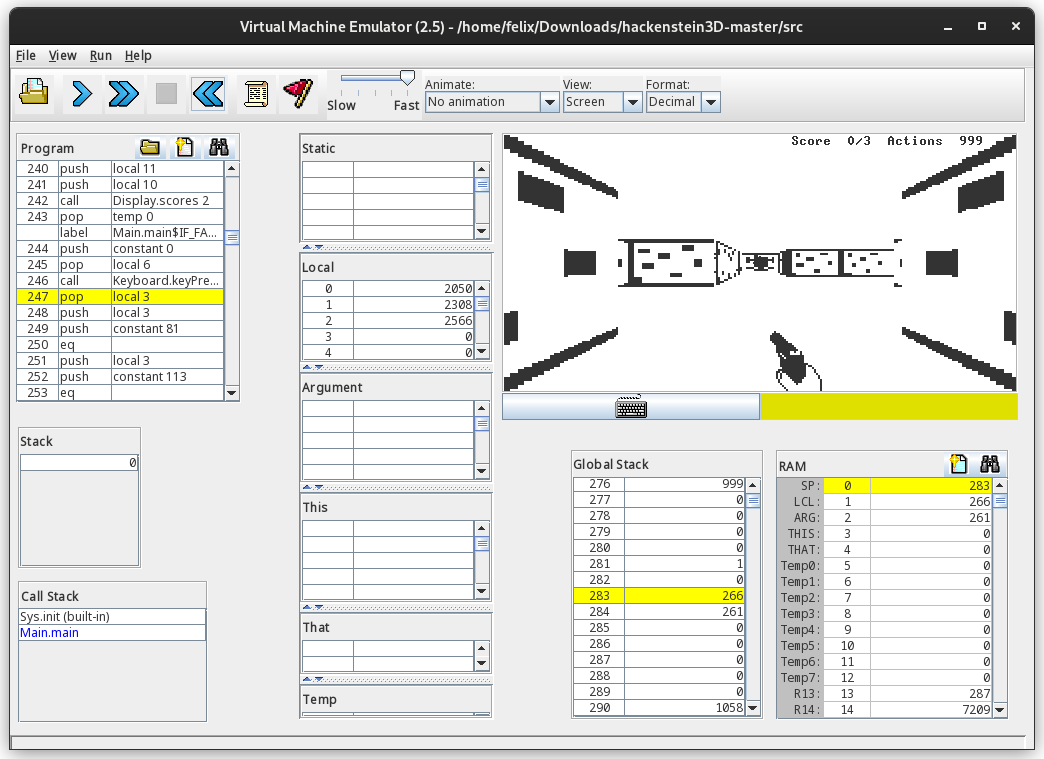
\includegraphics[width=14cm]{fig/hackenstein-offiziell.png}
    \caption{A simple Wolfenstein 3D Clone running in the VM Emulator}%
    \label{fig:hackenstein-offiziell}
  \end{figure}
\end{center}

\begin{center}
  \begin{figure}[h]
    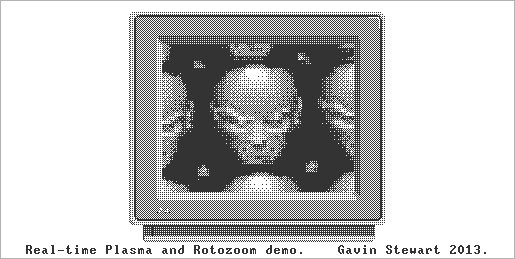
\includegraphics[width=14cm]{fig/gaschunky.png}
    \caption{A screenshot of the GASchunky animation in progress}%
    \label{fig:gaschunky-screenshot}
  \end{figure}
\end{center}

\section{Conclusions}
All things considered, the project was a success. The original goal of providing an alternative VM emulator implementation in the browser that is faster and better suited for modern displays was achieved.
Additionally, the CPU emulator was also rewritten and integrated into the same user interface, and the test script workflow was also ported to Rust.
Not everything is an improvement over the original emulator, however; there are still some opportunities for future improvements, as described in~\cref{future-work}.
All in all, the technologies chosen worked well to rewrite a complex desktop application for the modern web, and the potential of Wasm as a compilation target for such applications was demonstrated.
Further acceleration of the already existing trend of developing more and more applications for the web browser can be expected, as developers are now no longer limited to JavaScript or languages that can be compiled to it.

% \subsection{Summary}
% summary with emphasis on results/comparisons

\subsection{Future work} \label{future-work}
While the project resulted in a working application that fullfills the original goals, there are still multiple things that could be improved in the future.
First and foremost is the inclusion of the last of the three simulators, the hardware simulator. Since this simulator is not affected by performance issues, as only simple tests of the created logic gates are performed, it would benefit least from a rewrite in Rust. Having all of the simulators for the course inside of one single application would, however, be a great benefit for the students participating in the course as they would not have to install anything locally anymore.
This would require not just a new emulator to be written, but also a completely new user interface, while the VM and CPU can share a single interface due to their many similarities.
Another point that would greatly benefit the students would be the inclusion of further debugging tools, like breakpoints, more memory views~\ref{ui-showcase} and the inclusion of the test script runner into the web based user interface.
The last point is especially important, as those test scripts show the students that they correctly solved the problem before submitting their solutions.
Some minor improvements which could be made, are improved error messages and a compatibility mode for the keyboard handler.
The former should be relatively simple to implement, as the parsers already include the original source code location of each token in their output~\ref{spans}.
The latter point refers to something already discussed in~\cref{compatibility}. Instead of just emulating the behaviour of the official emulator perfectly, it might be useful to make the behaviour of the keyboard handler configurable for users.

% hardware simulator
% more debugging tools
% tst scripts in web ui
% proper error messages (spans already included)
% compatibility mode for keyboard uppercase

